%%%%%%%%%%%%%%%%%%%%%%%%%%%%%%%%%%%%%%%%%
% University/School Laboratory Report
% LaTeX Template
% Version 3.1 (25/3/14)
%
% This template has been downloaded from:
% http://www.LaTeXTemplates.com
%
% Original author:
% Linux and Unix Users Group at Virginia Tech Wiki 
% (https://vtluug.org/wiki/Example_LaTeX_chem_lab_report)
%
% License:
% CC BY-NC-SA 3.0 (http://creativecommons.org/licenses/by-nc-sa/3.0/)
%
%%%%%%%%%%%%%%%%%%%%%%%%%%%%%%%%%%%%%%%%%

%----------------------------------------------------------------------------------------
%	PACKAGES AND DOCUMENT CONFIGURATIONS
%----------------------------------------------------------------------------------------

\documentclass{article}

\usepackage[version=3]{mhchem} % Package for chemical equation typesetting
\usepackage{siunitx} % Provides the \SI{}{} and \si{} command for typesetting SI units
\usepackage{graphicx} % Required for the inclusion of images
\usepackage{natbib} % Required to change bibliography style to APA
\usepackage{amsmath} % Required for some math elements 
\usepackage{enumerate} % Required for the enumerate function
\usepackage[siunitx]{circuitikz} % Required for the drawing of circuit diagrams
\usepackage{caption}
\usepackage{graphicx}
\usepackage{subcaption}
\usepackage{xfrac}
\usepackage{float}
\usepackage{enumitem}
\usepackage{chemgreek}
\usepackage{pgfplots}
\usepackage{booktabs}
\usepackage[]{mcode}
\usepackage{epstopdf}

\setlength\parindent{0pt} % Removes all indentation from paragraphs

\renewcommand{\labelenumi}{\alph{enumi}.} % Make numbering in the enumerate environment by letter rather than number (e.g. section 6)

%\usepackage{times} % Uncomment to use the Times New Roman font

\graphicspath{{./fig/}}

%----------------------------------------------------------------------------------------
%	DOCUMENT INFORMATION
%----------------------------------------------------------------------------------------

\title{Communication Systems \\ Quadrature Amplitude Modulation \\ ENG473} % Title

\author{Shane \textsc{Reynolds}} % Author name

\date{\today} % Date for the report

\begin{document}

\maketitle % Insert the title, author and date

\begin{center}
\begin{tabular}{l r}
Date Performed: & October 09, 2016 \\ % Date the experiment was performed
Instructor: & Dr Sina Vafi % Instructor/supervisor
\end{tabular}
\end{center}

% If you wish to include an abstract, uncomment the lines below
% \begin{abstract}
% Abstract text
% \end{abstract}

%----------------------------------------------------------------------------------------
%	SECTION 1
%----------------------------------------------------------------------------------------

\section{Objective}

Verify the performance of Quadrature Amplitude Modulation (QAM). The experiment passes a randomly generated 30000 symbol binary stream through a simulated channel with Additive White Gaussian Noise to assess the performance of modulation and demodulation using QAM-16 with and without cyclic encoding.

%----------------------------------------------------------------------------------------
%	SECTION 2
%----------------------------------------------------------------------------------------

\section{Part 1: Process \& Results}
 Modulation allows us to take a baseband signal, like voice or music, and transmit it over a bandpass channel which attenuates higher and lower frequencies. In particular, the modulation process sees us multiply our signal, say $x(t)$, with a carrier signal which is in the form of a cosine function:
\begin{align}
	y(t) = x(t) \cdot \big(A_c \cdot \cos(\omega_c t + \phi_c)\big)
\end{align}

The parameters $A_c$, $\omega_c$ and $\phi_c$ are the parameters of the carrier signal, and we manipulate these in order the transmit the digital data along the carrier channel. The Quadrature carrier description is identical to the one shown above, except that we define our signal $x(t)$ as two components, the in-phase component, $x_i(t)$, and the quadrature component, $x_q(t)$. We thus redefine equation (1) as follows:
\begin{align}
	y(t) = A_c \cdot \big[x_i(t) \cdot \cos(\omega_c \cdot t + \phi_c) - x_q(t) \cdot \sin(\omega_c \cdot t + \phi_c)\big]
\end{align}

This provides us with an in-phase/quadrature plane in which we can specify locations for our symbols. This experiment focuses on 16 specific locations on the quadrature plane and distinguishes between them using the amplitude of the carrier signal, $A_c$. A random stream of 30000 binary bits are generated - a plot of the first 50 bits can be seen in Figure 1.

\begin{figure}[H]
	\hspace{-1.5cm}
	\begin{minipage}{7cm}
		\centering
		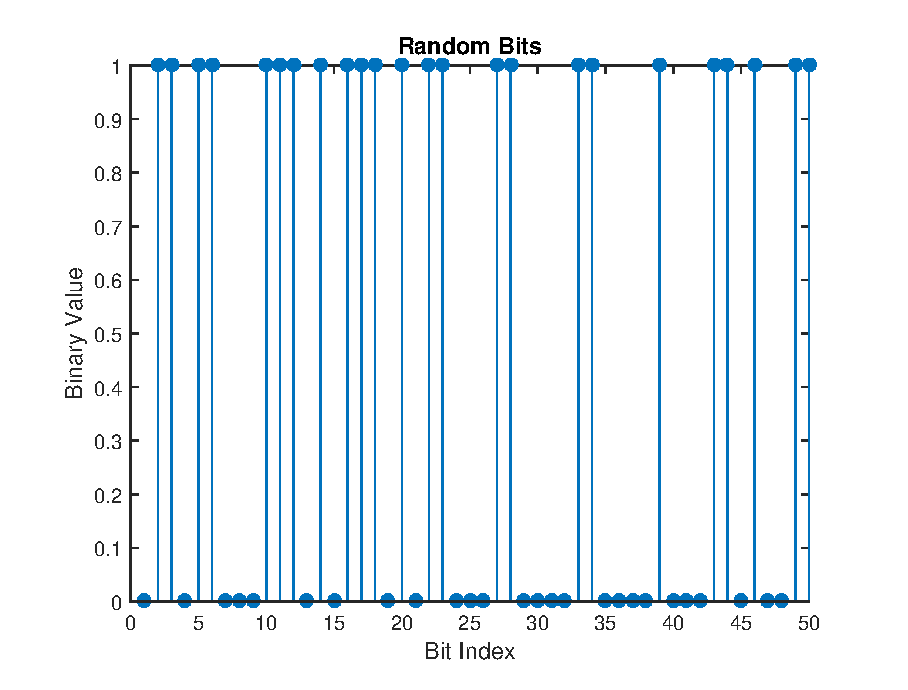
\includegraphics[scale=0.5]{figA}
		\caption{The first 50 random bits in the 30000 bit stream.}
	\end{minipage}
	\hspace{1cm}
	\begin{minipage}{7cm}
		\centering
		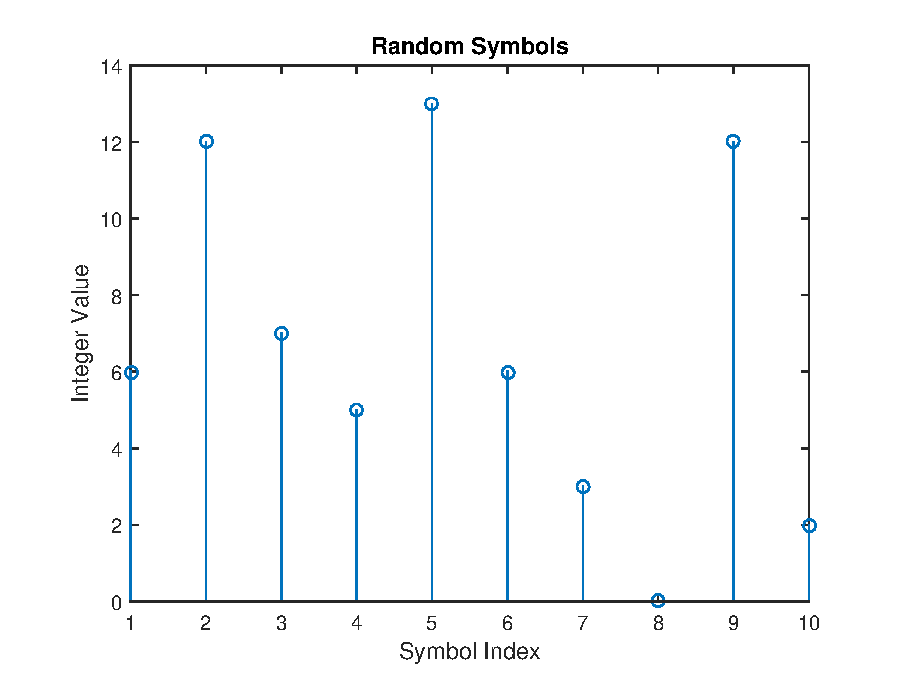
\includegraphics[scale=0.5]{figB}
		\caption{The first 10 4-bit symbols of the data for in preparation for modulation and transmission.}
	\end{minipage}
\end{figure}

In order to modulate the data stream with 16-QAM, the data streams need to be converted to 4-bit symbols - there are a total of 16 different permutations which we represent as a number from 1 to 16. A plot of the first 10 symbols can be seen in Figure 2.  

\begin{figure}[H]
	\centering
	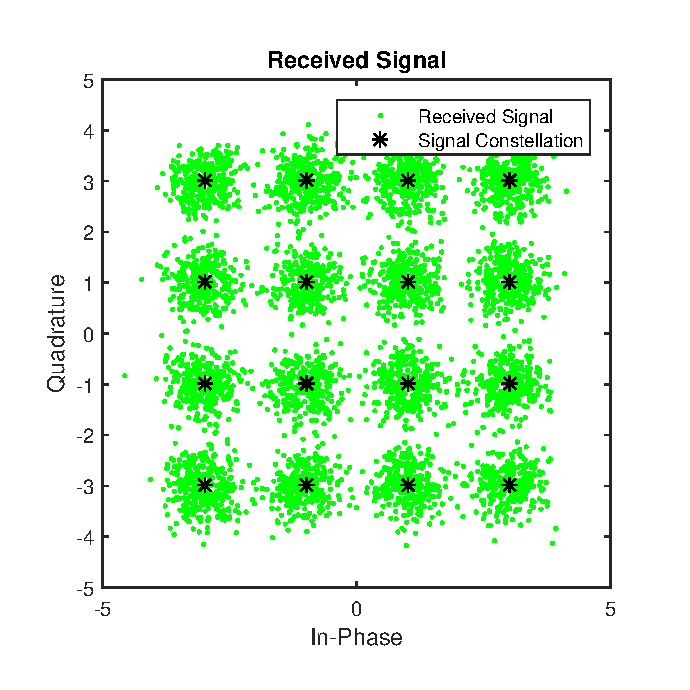
\includegraphics[scale=0.6]{figC}
	\caption{Signal constellation with received modulated data passed through noisy transmission channel.}
\end{figure}

 The data stream was modulated and passed through a simulated noisy channel. The simulated noise was Gaussian. The received signal can be seen in Figure 3 - the green dots represent the received data through the noisy channel and the black dots represent the actual signal constellation for the 16-QAM modulation scheme. The data was demodulated and the experiment repeated for different values of signal to noise ratio (SNR). The bit error ratio was calculated for each SNR value, the results of which can be seen in Table 1. Further, a plot of the data can be seen in Figure 4.

\begin{figure}[H]
	\hspace{-1.5cm}
	\begin{minipage}{6cm}
		\captionof{table}{16-QAM BER for received modulated data through noisy transmission channel for various SNR.}
		\begin{tabular}{rrrr}
			\toprule
			\textbf{SNR} ($\si{\decibel}$) & \textbf{BER} & \textbf{SNR} ($\si{\decibel}$) & \textbf{BER}\\
			\midrule
			6.0206&    0.1846 	& 	14.0206 	&    0.0124\\
			6.5206&    0.1713	& 	14.5206 	&    0.0086\\
			7.0206&    0.1574	& 	15.0206		&    0.0058\\
			7.5206&    0.1435	& 	15.5206		&    0.0038\\
			8.0206&    0.1301	&	16.0206		&    0.0024\\
			8.5206&    0.1164	&	16.5206		&    0.0014\\
			9.0206&    0.1031	&	17.0206		&    0.0008\\
			9.5206&    0.0905	&	17.5206		&    0.0004\\
			10.0206&    0.0782	&	18.0206		&    0.0002\\
			10.5206&    0.0667	&	18.5206		&    0.0001\\
			11.0206&    0.0560	&	19.0206		&    0.0000\\
			11.5206&    0.0459	&	19.5206		&    0.0000\\
			12.0206&    0.0372	&	20.0206		&    0.0000\\
			12.5206&    0.0293	&	20.5206		&    0.0000\\
			13.0206&    0.0226	&	21.0206		&    0.0000\\
			13.5206&    0.0170 & &\\
			\bottomrule
		\end{tabular}
	\end{minipage}
	\hspace{2cm}
	\begin{minipage}{6cm}
		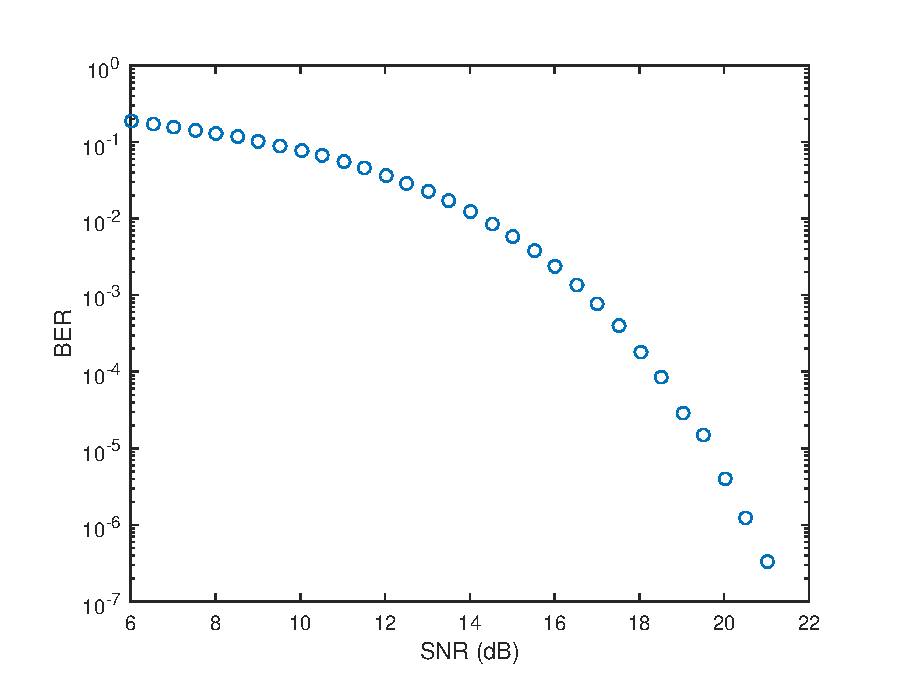
\includegraphics[scale=0.5]{fig1}
		\caption{BER of 16-QAM scheme for 30000-bit data stream, modulated in 4-bit words, for various values of SNR.}
	\end{minipage}
\end{figure}

%----------------------------------------------------------------------------------------
%	SECTION 3
%----------------------------------------------------------------------------------------

\section{Part 2: Process, Results \& Discussion}

\begin{table}[H]
	\centering
	\caption{text}
	\begin{tabular}{rrrr}
		\toprule
		\textbf{SNR} ($\si{\decibel}$) & \textbf{BER} & \textbf{SNR} ($\si{\decibel}$) & \textbf{BER}\\
		\midrule
		5.7744	&   23.4570	&	13.2744 &   2.6970\\
		6.2744  & 	22.0420	&	13.7744 &   1.9400\\
		6.7744  & 	20.4820	&	14.2744 &   1.3270\\
		7.2744  & 	18.8730	&	14.7744 &   0.9170\\
		7.7744  & 	16.8720	&	15.2744 &   0.5630\\
		8.2744  & 	15.4700	&	15.7744 &   0.3300\\
		8.7744  & 	14.1700	&	16.2744 &   0.1900\\
		9.2744  & 	12.2940	&	16.7744 &   0.1040\\
		9.7744  & 	10.5670	&	17.2744 &   0.0320\\
		10.2744 &   9.2560	&	17.7744 &   0.0430\\
		10.7744 &   8.0370	&	18.2744 &   0.0030\\
		11.2744 &   6.8200	&	18.7744 &   0.0040\\
		11.7744 &   5.5280	&	19.2744 &   0.0060\\
		12.2744 &   4.6530	&	19.7744 &        0\\
		\bottomrule
	\end{tabular}
\end{table}

\begin{figure}[H]
	\centering
	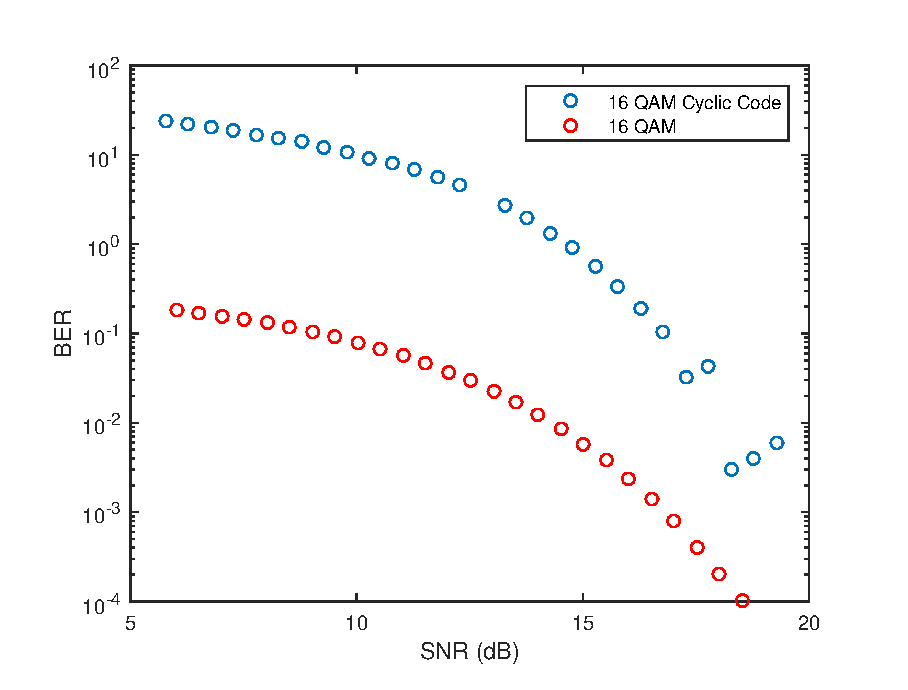
\includegraphics[scale=0.7]{fig2}
	\caption{text}
\end{figure}
%----------------------------------------------------------------------------------------
%	SECTION 5
%----------------------------------------------------------------------------------------

\section{Conclusion}



%----------------------------------------------------------------------------------------
%	APPENDIX A
%----------------------------------------------------------------------------------------

\section{Appendix A}



%----------------------------------------------------------------------------------------
%	APPENDIX B
%----------------------------------------------------------------------------------------

\section{Appendix B}



\end{document}